
\let\negmedspace\undefined
\let\negthickspace\undefined
\documentclass[journal,12pt,twocolumn]{IEEEtran}
%
\usepackage{setspace}
\usepackage{gensymb}
%\doublespacing
\singlespacing

%\usepackage{graphicx}
%\usepackage{amssymb}
%\usepackage{relsize}
\usepackage[cmex10]{amsmath}
%\usepackage{amsthm}
%\interdisplaylinepenalty=2500
%\savesymbol{iint}
%\usepackage{txfonts}
%\restoresymbol{TXF}{iint}
%\usepackage{wasysym}
\usepackage{amsthm}
%\usepackage{iithtlc}
\usepackage{mathrsfs}
\usepackage{txfonts}
\usepackage{stfloats}
\usepackage{steinmetz}
\usepackage{bm}
\usepackage{cite}
\usepackage{cases}
\usepackage{subfig}
%\usepackage{xtab}
\usepackage{longtable}
\usepackage{multirow}
%\usepackage{algorithm}
%\usepackage{algpseudocode}
\usepackage{enumitem}
\usepackage{mathtools}
\usepackage{tikz}
\usepackage{circuitikz}
\usepackage{verbatim}
\usepackage{tfrupee}
\usepackage[breaklinks=true]{hyperref}
%\usepackage{stmaryrd}
\usepackage{tkz-euclide} % loads  TikZ and tkz-base
%\usetkzobj{all}
\usepackage{listings}
    \usepackage{color}                                            %%
    \usepackage{array}                                            %%
    \usepackage{longtable}                                        %%
    \usepackage{calc}                                             %%
    \usepackage{multirow}                                         %%
    \usepackage{hhline}                                           %%
    \usepackage{ifthen}                                           %%
  %optionally (for landscape tables embedded in another document): %%
    \usepackage{lscape}     
\usepackage{multicol}
\usepackage{chngcntr}
%\usepackage{enumerate}
\usepackage{blkarray}
%\usepackage{wasysym}
%\newcounter{MYtempeqncnt}
\DeclareMathOperator*{\Res}{Res}
%\renewcommand{\baselinestretch}{2}
\renewcommand\thesection{\arabic{section}}
\renewcommand\thesubsection{\thesection.\arabic{subsection}}
\renewcommand\thesubsubsection{\thesubsection.\arabic{subsubsection}}

\renewcommand\thesectiondis{\arabic{section}}
\renewcommand\thesubsectiondis{\thesectiondis.\arabic{subsection}}
\renewcommand\thesubsubsectiondis{\thesubsectiondis.\arabic{subsubsection}}

% correct bad hyphenation here
\hyphenation{op-tical net-works semi-conduc-tor}
\def\inputGnumericTable{}                                 %%

\lstset{
%language=C,
frame=single, 
breaklines=true,
columns=fullflexible
}
%\lstset{
%language=tex,
%frame=single, 
%breaklines=true
%}

\begin{document}
%


\newtheorem{theorem}{Theorem}[section]
\newtheorem{problem}{Problem}
\newtheorem{proposition}{Proposition}[section]
\newtheorem{lemma}{Lemma}[section]
\newtheorem{corollary}[theorem]{Corollary}
\newtheorem{example}{Example}[section]
\newtheorem{definition}[problem]{Definition}
%\newtheorem{thm}{Theorem}[section] 
%\newtheorem{defn}[thm]{Definition}
%\newtheorem{algorithm}{Algorithm}[section]
%\newtheorem{cor}{Corollary}
\newcommand{\BEQA}{\begin{eqnarray}}
\newcommand{\EEQA}{\end{eqnarray}}
\newcommand{\define}{\stackrel{\triangle}{=}}

\bibliographystyle{IEEEtran}
%\bibliographystyle{ieeetr}


\providecommand{\mbf}{\mathbf}
\providecommand{\pr}[1]{\ensuremath{\Pr\left(#1\right)}}
\providecommand{\qfunc}[1]{\ensuremath{Q\left(#1\right)}}
\providecommand{\sbrak}[1]{\ensuremath{{}\left[#1\right]}}
\providecommand{\lsbrak}[1]{\ensuremath{{}\left[#1\right.}}
\providecommand{\rsbrak}[1]{\ensuremath{{}\left.#1\right]}}
\providecommand{\brak}[1]{\ensuremath{\left(#1\right)}}
\providecommand{\lbrak}[1]{\ensuremath{\left(#1\right.}}
\providecommand{\rbrak}[1]{\ensuremath{\left.#1\right)}}
\providecommand{\cbrak}[1]{\ensuremath{\left\{#1\right\}}}
\providecommand{\lcbrak}[1]{\ensuremath{\left\{#1\right.}}
\providecommand{\rcbrak}[1]{\ensuremath{\left.#1\right\}}}
\theoremstyle{remark}
\newtheorem{rem}{Remark}
\newcommand{\sgn}{\mathop{\mathrm{sgn}}}
\providecommand{\abs}[1]{\left\vert#1\right\vert}
\providecommand{\res}[1]{\Res\displaylimits_{#1}} 
\providecommand{\norm}[1]{\left\lVert#1\right\rVert}
%\providecommand{\norm}[1]{\lVert#1\rVert}
\providecommand{\mtx}[1]{\mathbf{#1}}
\providecommand{\mean}[1]{E\left[ #1 \right]}
\providecommand{\fourier}{\overset{\mathcal{F}}{ \rightleftharpoons}}
%\providecommand{\hilbert}{\overset{\mathcal{H}}{ \rightleftharpoons}}
\providecommand{\system}{\overset{\mathcal{H}}{ \longleftrightarrow}}
	%\newcommand{\solution}[2]{\textbf{Solution:}{#1}}
\newcommand{\solution}{\noindent \textbf{Solution: }}
\newcommand{\cosec}{\,\text{cosec}\,}
\providecommand{\dec}[2]{\ensuremath{\overset{#1}{\underset{#2}{\gtrless}}}}
\newcommand{\myvec}[1]{\ensuremath{\begin{pmatrix}#1\end{pmatrix}}}
\newcommand{\mydet}[1]{\ensuremath{\begin{vmatrix}#1\end{vmatrix}}}
%\numberwithin{equation}{section}
\numberwithin{equation}{subsection}
%\numberwithin{problem}{section}
%\numberwithin{definition}{section}
\makeatletter
\@addtoreset{figure}{problem}
\makeatother

\let\StandardTheFigure\thefigure
\let\vec\mathbf
%\renewcommand{\thefigure}{\theproblem.\arabic{figure}}
\renewcommand{\thefigure}{\theproblem}
%\setlist[enumerate,1]{before=\renewcommand\theequation{\theenumi.\arabic{equation}}
%\counterwithin{equation}{enumi}


%\renewcommand{\theequation}{\arabic{subsection}.\arabic{equation}}

\def\putbox#1#2#3{\makebox[0in][l]{\makebox[#1][l]{}\raisebox{\baselineskip}[0in][0in]{\raisebox{#2}[0in][0in]{#3}}}}
     \def\rightbox#1{\makebox[0in][r]{#1}}
     \def\centbox#1{\makebox[0in]{#1}}
     \def\topbox#1{\raisebox{-\baselineskip}[0in][0in]{#1}}
     \def\midbox#1{\raisebox{-0.5\baselineskip}[0in][0in]{#1}}

\vspace{3cm}

\title{
	%\logo{
Matrix Analysis
	%}
}
\author{ G V V Sharma$^{*}$% <-this % stops a space
	\thanks{*The author is with the Department
		of Electrical Engineering, Indian Institute of Technology, Hyderabad
		502285 India e-mail:  gadepall@iith.ac.in. All content in this manual is released under GNU GPL.  Free and open source.}
	
}	
%\title{
%	\logo{Matrix Analysis through Octave}{\begin{center}\includegraphics[scale=.24]{tlc}\end{center}}{}{HAMDSP}
%}


% paper title
% can use linebreaks \\ within to get better formatting as desired
%\title{Matrix Analysis through Octave}
%
%
% author names and IEEE memberships
% note positions of commas and nonbreaking spaces ( ~ ) LaTeX will not break
% a structure at a ~ so this keeps an author's name from being broken across
% two lines.
% use \thanks{} to gain access to the first footnote area
% a separate \thanks must be used for each paragraph as LaTeX2e's \thanks
% was not built to handle multiple paragraphs
%

%\author{<-this % stops a space
%\thanks{}}
%}
% note the % following the last \IEEEmembership and also \thanks - 
% these prevent an unwanted space from occurring between the last author name
% and the end of the author line. i.e., if you had this:
% 
% \author{....lastname \thanks{...} \thanks{...} }
%                     ^------------^------------^----Do not want these spaces!
%
% a space would be appended to the last name and could cause every name on that
% line to be shifted left slightly. This is one of those "LaTeX things". For
% instance, "\textbf{A} \textbf{B}" will typeset as "A B" not "AB". To get
% "AB" then you have to do: "\textbf{A}\textbf{B}"
% \thanks is no different in this regard, so shield the last } of each \thanks
% that ends a line with a % and do not let a space in before the next \thanks.
% Spaces after \IEEEmembership other than the last one are OK (and needed) as
% you are supposed to have spaces between the names. For what it is worth,
% this is a minor point as most people would not even notice if the said evil
% space somehow managed to creep in.



% The paper headers
%\markboth{Journal of \LaTeX\ Class Files,~Vol.~6, No.~1, January~2007}%
%{Shell \MakeLowercase{\textit{et al.}}: Bare Demo of IEEEtran.cls for Journals}
% The only time the second header will appear is for the odd numbered pages
% after the title page when using the twoside option.
% 
% *** Note that you probably will NOT want to include the author's ***
% *** name in the headers of peer review papers.                   ***
% You can use \ifCLASSOPTIONpeerreview for conditional compilation here if
% you desire.




% If you want to put a publisher's ID mark on the page you can do it like
% this:
%\IEEEpubid{0000--0000/00\$00.00~\copyright~2007 IEEE}
% Remember, if you use this you must call \IEEEpubidadjcol in the second
% column for its text to clear the IEEEpubid mark.



% make the title area
\maketitle

\newpage

\tableofcontents

\bigskip

\renewcommand{\thefigure}{\theenumi}
\renewcommand{\thetable}{\theenumi}
%\renewcommand{\theequation}{\theenumi}

%\begin{abstract}
%%\boldmath
%In this letter, an algorithm for evaluating the exact analytical bit error rate  (BER)  for the piecewise linear (PL) combiner for  multiple relays is presented. Previous results were available only for upto three relays. The algorithm is unique in the sense that  the actual mathematical expressions, that are prohibitively large, need not be explicitly obtained. The diversity gain due to multiple relays is shown through plots of the analytical BER, well supported by simulations. 
%
%\end{abstract}
% IEEEtran.cls defaults to using nonbold math in the Abstract.
% This preserves the distinction between vectors and scalars. However,
% if the journal you are submitting to favors bold math in the abstract,
% then you can use LaTeX's standard command \boldmath at the very start
% of the abstract to achieve this. Many IEEE journals frown on math
% in the abstract anyway.

% Note that keywords are not normally used for peerreview papers.
%\begin{IEEEkeywords}
%Cooperative diversity, decode and forward, piecewise linear
%\end{IEEEkeywords}



% For peer review papers, you can put extra information on the cover
% page as needed:
% \ifCLASSOPTIONpeerreview
% \begin{center} \bfseries EDICS Category: 3-BBND \end{center}
% \fi
%
% For peerreview papers, this IEEEtran command inserts a page break and
% creates the second title. It will be ignored for other modes.
%\IEEEpeerreviewmaketitle

\begin{abstract}
This book provides a computational approach to school geometry based on the NCERT textbooks from Class 6-12.  Links to sample Python codes are available in the text.  
\end{abstract}
Download python codes using 
\begin{lstlisting}
svn co https://github.com/gadepall/school/trunk/ncert/computation/codes
\end{lstlisting}

\section{Examples}
\renewcommand{\theequation}{\theenumi}
\begin{enumerate}[label=\thesection.\arabic*.,ref=\thesection.\theenumi]
\numberwithin{equation}{enumi}

\input{./line/chem.tex}
\input{./line/matrix_exam.tex}
%\renewcommand{\theequation}{\theenumi}
%\begin{enumerate}[label=\arabic*.,ref=\thesubsection.\theenumi]
%\numberwithin{equation}{enumi}

\item Find 
$\begin{vmatrix}
2&4\\-5&-1
\end{vmatrix}$
\\
\solution 
\input{./solutions/1/chapters/line/det/solution.tex}

\item (i) $\begin{vmatrix}\cos\theta& -\sin\theta\\ \sin\theta& \cos\theta \end{vmatrix}$ 
(ii) $\begin{vmatrix}
x^2-x+1& x-1\\ x+1&  x+1
\end{vmatrix}$
\\
\solution 
\input{./solutions/2/chapters/line_ex/determinants/solution.tex}
\item If$ \vec{A} = \begin{vmatrix}1&2\\4&2\end{vmatrix}$,then show that  
$\abs{2\vec{A}}=4\abs{\vec{A}}$
\\
\solution 
\input{./solutions/3/chapters/line/det/solution.tex}
\item If $\vec{A}=\begin{vmatrix}1&0&1\\0&1&2\\0&0&4\end{vmatrix}$, then show that $\abs{3\vec{A}}=27\abs{\vec{A}}$
\\
\solution 
\input{./solutions/4/chapters/line/determinent/solution.tex}
\item Evaluate the determinants
\begin{enumerate}
\item $\begin{vmatrix}
3&-1&-2\\0&0&-1\\3&-5&0
\end{vmatrix}$
\item $\begin{vmatrix}
3&-4&5\\1&1&-2\\2&3&1
\end{vmatrix}$
\\
\solution 
\input{./solutions/5/chapters/lines/docq14.tex}
\item $\begin{vmatrix}
0&1&2 \\ -1&0&-3\\-2&3&0
\end{vmatrix}$
\item $\begin{vmatrix}
2&-1&-2\\0&2&-1\\3&-5&0
\end{vmatrix}$
\end{enumerate}  
\item If A=$\begin{vmatrix}1&1&-2\\2&1&-3\\5&4&-9\end{vmatrix}$, 
find $\abs{A}$
\\
\solution 
\input{./solutions/6/chapters/line/determinants/solution.tex}
\item Find the values of x,If\\
(i)$\begin{vmatrix}
2&4\\5&1
\end{vmatrix}$ =$\begin{vmatrix}
2x&4 \\ 6&x
\end{vmatrix}$
(ii)$\begin{vmatrix}
2&3 \\ 4&5
\end{vmatrix}$ =$\begin{vmatrix}
x&3 \\ 2x&5
\end{vmatrix}$
\\
\solution 
\input{./solutions/7/chapters/line/det/solution.tex}
\item If  $\begin{vmatrix}
x&2 \\ 18&x
\end{vmatrix}$ =$\begin{vmatrix}
6&2 \\ 18&6
\end{vmatrix}$, then x is equal to 
\begin{enumerate}
\item 6
\item $\pm 6$
\item $-6$
\item 0
\end{enumerate}
\item $\begin{vmatrix}
x&a&x+a\\y&b&y+b\\z&c&z+c\end{vmatrix}=0$
\\
\solution 
\input{./solutions/det/9/solution.tex}
\item $\begin{vmatrix}
a-b&b-c&c-a\\b-c&c-a&a-b\\c-a&a-b&b-c\end{vmatrix}=0$
\\
\solution 
\input{./solutions/det/10/solution.tex}
\item $\begin{vmatrix}2&7&65\\3&8&75\\5&9&86\end{vmatrix}=0$
\\
\solution 
\input{./solutions/det/11/latex/solution.tex}
\item $\begin{vmatrix}1&bc&a(b+c)\\1&ca&b(c+a)\\1&ab&c(a+b)\end{vmatrix}=0$
\\
\solution 
\input{./solutions/det/12/solution.tex}
\item $\begin{vmatrix}b+c& q+r& y+z\\c+a& r+p& z+x\\a+b& p+q& x+y\end{vmatrix}$=2$\begin{vmatrix} a&p&x\\b&q&y\\c&r&z\end{vmatrix}$ 
\\
\solution 
\input{./solutions/det/13/solution.tex}
\item $\begin{vmatrix}-a^2&ab&ab\\ ba&-b^2&bc\\ ca&cb&-c^2\end{vmatrix}$=$4a^2b^2c^2$\\
\\
\solution 
\input{./solutions/det/15/solution.tex}
By Using properties of determinants, in Exercises 16 to 22,Show that;
\item (i)$\begin{vmatrix}1&a&a^2\\1&b&b^2\\1&c&c^2\end{vmatrix}$=(a-b)(b-c)(c-a)\\
(ii) $\begin{vmatrix}1&1&1 \\ a&b&c \\ a^3&b^3&c^3\end{vmatrix}$=(a-b)(b-c)(c-a)(a+b+c)
\\
\solution 
\input{./solutions/det/16_2/latex/solution.tex}
\item $\begin{vmatrix}x&x^2&yz \\ y&y^2&zx \\ z&z^2&xy\end{vmatrix}$=(x-y)(y-z)(z-x)(xy+yz+zx)
\item (i) $\begin{vmatrix}x+4&2x&2x \\ 2x&x+4&2x \\ 2x&2x&x+4\end{vmatrix}$=$(5x+4)(4-x)^2$\\
\solution 
\input{./solutions/det/18_1/solution.tex}
(ii) $\begin{vmatrix}y+k&y&y \\ y&y+k&y \\ y&y&xy+k\end{vmatrix}$=$k^2(3y+k)$
\\
\solution 
\input{./solutions/det/18_2/solution.tex}

\item $\begin{vmatrix}a^2+1&ab&ac \\ ab&b^2+1&bc \\ ca&cb&c^2+1\end{vmatrix}$=$1+a^2+b^2+c^2$\\
\\
\solution 
\input{./solutions/det/22/solution.tex}
Choose the correct answer in Exercises 23 and 24.
\item Let A be a square matrix of order 3X3, then 
$\abs{kA}$ is equal to
\begin{enumerate}
\item $k\abs{A}$
\item $k^2\abs{A}$
\item $k^3\abs{A}$
\item $3k\abs{A}$
\end{enumerate} 
\item Which of the following is correct
\begin{enumerate}
\item Determinant is a square matrix.
\item Determinant is a number associated to a matrix.
\item Determinant is a number associated to a square matrix.
\item None of these.
\end{enumerate}
\item Find area of the triangle with vertices at the point given in each of the following :\\
(i) \myvec{1&0}, \myvec{6&0}, \myvec{4&3}\\
(ii) \myvec{2&7}, \myvec{1&1}, \myvec{10&8}\\
(iii) \myvec{-2&-3}, \myvec{3&2}, \myvec{-1&-8}\\
\solution 
\begin{enumerate}
    \item 
    
Let the given Matrix be
\begin{equation}
\vec{A} = \myvec{3&5\\1&1}
\end{equation}
Transposing the above matrix gives,
\begin{equation}
\vec{A}^{\top} = \myvec{3&1\\5&1}
\end{equation}
Now, for Symmetric and Skew Symmetric Matrix,
\begin{align}
    \vec{B} &= \frac{\vec{A} + \vec{A}^{\top}}{2} = \myvec{3&3\\3&1} \\
    &= \vec{B}^{\top}
\end{align}
Also,
\begin{align}
    \vec{C} &= \frac{\vec{A} - \vec{A}^{\top}}{2} = \myvec{0&2\\-2&0} \\
    &= -\vec{C}^{\top}
\end{align}

Hence, $\vec{B}$ is a Symmetric Matrix and $\vec{C}$ is a Skew Symmetric Matrix and $\vec{B} + \vec{C} = \vec{A}$.
\begin{align}
    \therefore \myvec{3&5\\1&1} = \myvec{3&3\\3&1} + \myvec{0&2\\-2&0}  
\end{align}




    

\end{enumerate}
\item Show that points A=\myvec{a&b+c}, B=\myvec{b&c+a}, C=\myvec{c&a+b} are collinear.
\\
\solution 
\input{./solutions/det/26/solution.tex}
\item Find values of k if area of triangle is 4sq.units and vertices are \\
(i)) \myvec{k&0}, \myvec{4&0}, \myvec{0&2} \\ (ii) \myvec{-2&0}, \myvec{0&4}, \myvec{0&k}
\item Find equation of line joining
\begin{enumerate}
\item  \myvec{1&2} and \myvec{3&6} 
\item \myvec{3&1} and \myvec{9&3}.
\end{enumerate}
\solution
\begin{enumerate}
    \item Let 
\begin{align}
    \vec{A}= \myvec{x\\-1} , \vec{B} = \myvec{2\\1} , \vec{C} = \myvec{4\\5}
\end{align}

Now,
\begin{align}
    \vec{B}-\vec{A} & = \myvec{2-x\\1-(-1)}\\
                    & = \myvec{2-x\\2}
\end{align}
\begin{align}
    \vec{B}-\vec{C} & = \myvec{2-4\\1-5}\\
                    & = \myvec{-2\\-4}
\end{align}

Forming the matrix $\vec{M}$,
\begin{align}
    \vec{M} & = \myvec{\vec{B}-\vec{A}  &  \vec{B}-\vec{C}}^\top \\
            & =\myvec{2-x & 2\\2 & -4}^\top\\
            & = \myvec{2-x & 2 \\ -2 & -4}
\end{align}

Using matrix transformation,


\begin{align}
 \vec{M} = \myvec{2-x & 2\\-2 & -4}
 \xleftrightarrow{\text{$R_2$}\rightarrow{\text{$R_2/2$}}} 
 \myvec{2-x & 2 \\-1 & -2}\\
 \xleftrightarrow{\text{$R_2$}\rightarrow{\text{$R_2 + R_1$}}}
 \myvec{2-x & 2 \\1-x & 0}
\end{align}
\begin{align}
 rank(\vec{M}) = 1 &\implies  R_2 =0 \\
 \text{or, }
            x=1
\end{align}
See Fig.          \ref{aug/2/9/plot}.
\begin{figure}[!h]
         \centering
         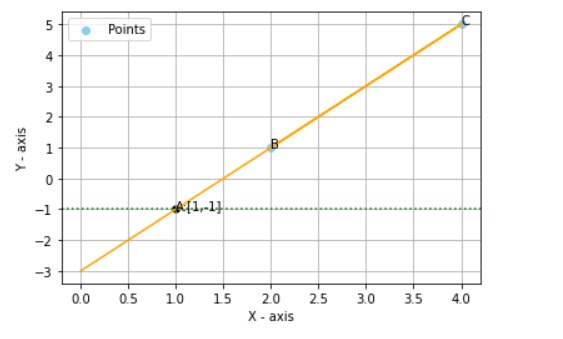
\includegraphics[width=\columnwidth]{solutions/aug/2/9/figures/figure.jpeg}
         \caption{Plot of the line }
         \label{aug/2/9/plot}
\end{figure}




    \item Let 
	\begin{align}
	 \vec{A} = \myvec{1\\2} , \vec{B} = \myvec{3 \\ 6}
	\end{align}
The direction vector 
\begin{align}
\vec{m}&= \vec{B}-\vec{A}=\myvec{2\\4}
\\
\implies 
    \vec{n}&= \myvec{-4\\2}
\end{align}
and 
\begin{align}
    c = \vec{n}^\top \vec {A} = \myvec{-4&2} \myvec{1\\2}=0 
\end{align}
This is verified in Fig. \ref{aug/76/2/fig:1}.
\begin{figure}[!ht]
\centering
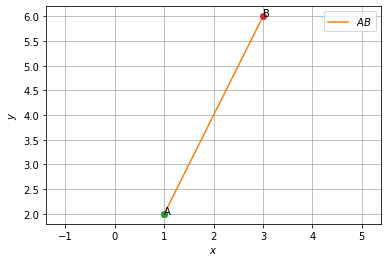
\includegraphics[width=\columnwidth]{solutions/aug/1/76/2/fig5.png}
\caption{LINE AB}
\label{aug/76/2/fig:1}
\end{figure}

    
\end{enumerate}

\item If the area of triangle is 35 sq.units with vertices \myvec{2&-6}, \myvec{5&4} and \myvec{k&4}.then k is 
\begin{enumerate}
\item 12
\item -2
\item -12,-2
\item 12,-2
\end{enumerate}
\solution
Let
\begin{align}
   \vec{A} = \myvec{2\\-6} , \vec{B} = \myvec{5 \\ 4}, \vec{C} = \myvec{k\\4} 
\end{align}
From the given information,
%
\begin{align}
   \frac{1}{2}\myvec{1 & 1& 1 \\
   \vec{A}&\vec{B}&\vec{C}}
   &= \mydet{
    1 & 1 & 1 \\ 
    2 & 5 & k \\ 
    -6 & 4 & 4} \\ &= 35
\end{align}
Simplifying the determinant, 
\begin{align}
   \mydet{1 & 1 & 1  \\ 
 2 & 5 & k \\ 
-6 & 4 & 4}
\xleftrightarrow [C_2-C_3\rightarrow C_2]{C_1-C_3\rightarrow C_1}
 \mydet{0 & 0 & 1  \\ 
 2-k & 5-k & k \\ 
10 & 0 & 4}
\end{align}
which upon expanding the cofactor yields
\begin{align}
     \mydet{2-k & 5-k \\ 
10 & 0 } = 10(5-k)
\end{align}
Thus, 
\begin{align}
   \frac{1}{2}10(5-k) &= 35
\\
  \implies  k &= -2
\end{align}

\textbf{Write Minors and Coafactors of the elements of following determinants:}
\item (i) $\begin{vmatrix}
2&-4 \\ 0 &3 \end{vmatrix}$ \\
(ii) $\begin{vmatrix}a&c \\ b &d\end{vmatrix}$
\item (i) $\begin{vmatrix}1&0&0 \\ 0&1&0 \\ 0&0&1\end{vmatrix}$\\
(ii) $\begin{vmatrix}1&0&4 \\ 3&5&-1 \\ 0&1&2\end{vmatrix}$
\item Using Cofactors of elements of second row,evaluate $\Delta$ =
$\begin{vmatrix} 5&3&8 \\ 2&0&1 \\ 1&2&3 \end{vmatrix}.$
\item Using Cofactors of elements of third column ,evaluate $\Delta$ = 
$\begin{vmatrix} 1&x&yz \\ 1&y&zx \\ 1&z&xy \end{vmatrix}.$
\item If $\Delta = \begin{vmatrix}
a_{11}&a_{12}&a_{13} \\ a_{21}&a_{22}&a_{23} \\ a_{31}&a_{32}&a_{33}
\end{vmatrix}$ and $A_{ij}$ is Cofactors of $a_{ij}$ then value of $\Delta$ is given by 
\begin{enumerate}
\item $a_{11}A_{31}+a_{12}A_{32}+a_{13}A_{33}$
\item $a_{11}A_{11}+a_{12}A_{21}+a_{13}A_{31}$
\item $a_{21}A_{11}+a_{22}A_{12}+a_{23}A_{13}$
\item $a_{11}A_{11}+a_{21}A_{21}+a_{31}A_{31}$
\end{enumerate} 
\textbf{Find adjoint of each of the matrices} 
\item $\begin{bmatrix}
1&2 \\ 3&4
\end{bmatrix}$
\item $\begin{bmatrix}
1&-1&2 \\ 2&3&5 \\ -2&0&1
\end{bmatrix}$
Verify A(adjA)=(adjA)A=$\abs{A}I$
\item $\begin{bmatrix}
2&3 \\ -4&-6
\end{bmatrix}$
\item $\begin{bmatrix}
1&-1&2 \\ 3&0&-2 \\ 1&0&3
\end{bmatrix}$
\item $\begin{bmatrix}
2&-2 \\ 4&3
\end{bmatrix}$
\item $\begin{bmatrix}
-1&5 \\ -3&2
\end{bmatrix}$
\item $\begin{bmatrix}
1&2&3 \\ 0&2&4 \\ 0&0&5
\end{bmatrix}$
\item $\begin{bmatrix}
1&0&0 \\ 3&3&0 \\ 5&2&-1
\end{bmatrix}$
\item $\begin{bmatrix}
2&1&3 \\ 4&-1&0 \\ -7&2&1
\end{bmatrix}$
\item $\begin{bmatrix}
1&-1&2 \\ 0&2&-3 \\ 3&-2&4
\end{bmatrix}$
\item $\begin{bmatrix}
1&0&0 \\ 0& \cos\alpha &\sin\alpha \\ 0&\sin\alpha&-\cos\alpha
\end{bmatrix}$
\item Let A=
$\begin{bmatrix}
3&7 \\ 2&5
\end{bmatrix}$ and B=
$\begin{bmatrix}
6&8 \\ 7&9
\end{bmatrix}.$ Verify that $(AB)^{-1}=B^{-1} A^{-1}$
\item Let A =$\begin{bmatrix}
3&1 \\ -1&2
\end{bmatrix},$ show that $A^2-5A+7I=O.$ Hence find $A^{-1}$
\solution 
\input{./solutions/det/47/solution.tex}
\item For the matrix A= $\begin{bmatrix}
3&2 \\ 1&1
\end{bmatrix},$ find the numbers a and b such that $A^2+aA+bI=O.$
\\
\solution 
\input{./solutions/det/48/solution.tex}

\item For the matrix A=$\myvec{1&1&1 \\ 1&2&-3 \\ 2&-1&3}$.Show that \begin{align}
    A^3-6A^2+5A+11I=0\label{eq:det/49/1}
\end{align} and hence find $A^{-1}$.
%\item For the matrix A=$\begin{bmatrix}
%1&1&1 \\ 1&2&-3 \\ 2&-1&3
%\end{bmatrix}$ Show that $A^3-6A^2+9A-4I=O$ and hence find $A^{-1}$
\solution 
\input{./solutions/det/49/solution.tex}
\item Let A be a nonsingular square matrix of order 3X3 .Then $\abs{adjA}$ is equal to 
\begin{enumerate}
\item $\abs{A}$
\item $\abs{A}^2$
\item $\abs{A}^3$
\item $3\abs{A}$
\end{enumerate}
\item If A is an invertible matrix of order 2, then det($A^{-1}$) is equal to 
\begin{enumerate}
\item det(A)
\item $\frac{1}{det(A)}$
\item 1
\item 0
\end{enumerate}
\textbf{Examine the consistency of the system of given Equations.}
\item $\begin{alignedat}[t]{2}
x+3y&=5 
\\
2x+6y&=8 
\end{alignedat}$\\
\\
\solution 
\input{./solutions/det/54/solution.tex}
\item x+y+z=1\\ 2x+3y+2z=2\\ax+ay+2az=4\\
\\
\solution 
\input{./solutions/det/55/latex/solution.tex}
\item 3x-y-2z=2 \\ 2y-z=-1 \\ 3x-5y=3\\
\\
\solution 
\input{./solutions/det/56/solution.tex}
\item 5x-y+4z=5 \\ 2x+3y+5z=2 \\ 5x-2y+6z=-1\\
\\
\solution
\input{./solutions/det/57/solution.tex}
Solve the system linear equations,using matrix method.
\item 
$\begin{alignedat}[t]{2}
%\myvec{5 & 2}\vec{x} &= 4
%\\ 
%\myvec{7 & 3}\vec{x} &= 5
5x+2y&=4 \\ 7x+3y&=5
\end{alignedat}$
\\
\solution
\input{./solutions/det/58/solution.tex}
\item 
$\begin{alignedat}[t]{2}
%\myvec{2 & -1}\vec{x} &= -2
%\\ 
%\myvec{3 & 4}\vec{x} &= 3
2x-y&=-2 \\ 3x+4y&=3
\end{alignedat}$
\\
\solution
\input{./solutions/det/59/solution.tex}
\item $\begin{alignedat}[t]{2}
%\myvec{4 & -3}\vec{x} &= 3
%\\ 
%\myvec{3 & -5}\vec{x} &= 7
4x-3y&=3 \\ 3x-5y&=7
\end{alignedat}$
\\
\solution
\input{./solutions/det/60/solution.tex}
\item $\begin{alignedat}[t]{2}
%\myvec{5 & 2}\vec{x} &= 3
%\\ 
%\myvec{3 & 2}\vec{x} &= 5
5x+2y&=3 \\ 3x+2y&=5
\end{alignedat}$\\
\\
\solution
\input{./solutions/det/61/solution.tex}
\item 2x+y+z = 1 \\ x-2y-z = $\frac{3}{2}$ \\ 3y- 5z = 9\\
\item x-y+z = 4 \\ 2x+y-3z = 0 \\ x+y+z = 2\\
\item 2x+3y+3z = 5 \\ x-2y+z = -4 \\ 3x-y-2z = 3\\
\item x-y+2z = 7 \\ 3x+4y-5z = -5 \\ 2x-y+3z = 12\\ 
\item If A=$\begin{bmatrix}
2&-3&5 \\ 3&2&-4 \\ 1&1&-2
\end{bmatrix},$ find $A^{-1}.$ Using $A^{-1}$ solve the system of equations \\
2x-3y+5z = 11, \\ 3x+2y-4z = -5, \\ x+y-2z =-3.\\
\item The cost of 4 kg onion, 3 kg wheat and 2 kg rice is \rupee 60. The cost of 2 kg onion,4 kg wheat and 6 kg rice is \rupee 90.The cost of 6kg onion 2kg wheat and 3kg rice is \rupee 70.Find the cost of each item per kg by matrix mathod. 
\item Prove that the determinant \\
$\begin{vmatrix}
x &\sin\theta&\cos\theta \\ -\sin\theta&-x&1 \\ \cos\theta&1&x
\end{vmatrix}$ 
is independent of $\theta$
\\
\solution 
\input{./solutions/det/68/solution.tex}

\item Without expanding the determinant, prove that\\ $\begin{vmatrix}
a&a^2&bc \\ b&b^2&ca \\c&c^2&ab
\end{vmatrix}=\begin{vmatrix}
1&a^2&a^3 \\ 1&b^2&b^3 \\ 1&c^2&c^3
\end{vmatrix}$.
\\
\solution
%\input{./solutions/det/69/solution.tex}
\item Evaluate 
$\begin{vmatrix}
\cos\alpha \cos\beta &\cos\alpha \sin\beta &-\sin\alpha \\ -\sin\beta & \cos\beta &0 \\ \sin\alpha\cos\beta&\sin\alpha\sin\beta&\cos\alpha
\end{vmatrix}.$\\
\solution 
\input{./solutions/det/70/solution.tex}
\item If a,b and c are real numbers, and \\$\Delta=\begin{vmatrix}
b+c&c=a&a=b \\ c+a&a+b&b+c \\ a+b&b+c&c+a
\end{vmatrix}=0,$ Show that either a+b+c=0 or a=b=c.\\
\solution 
\input{./solutions/det/71/solution.tex}
\item Solve the equation\\ $\begin{vmatrix}
x+a&x&x \\ x&x+a&x \\ x&x&x+a
\end{vmatrix}=0, a\neq0$\\
\solution 
\input{./solutions/det/72/solution.tex}
\item Prove that \\
$\begin{vmatrix}
a^2&bc&ac+c^2 \\ a^2+ab&b^2&ac \\ab&b^2+bc&c^2
\end{vmatrix}= 4a^2b^2c^2$\\
\solution 
\input{./solutions/det/73/solution.tex}
\item If \\
$A^{-1}=\begin{bmatrix}
3&-1&1 \\ -15&6&-5 \\5&-2&2
\end{bmatrix}$ and B=$\begin{bmatrix}
1&2&-2 \\ -1&3&0 \\0&-2&1
\end{bmatrix},$ find $(AB)^{-1}$\\
\item Let A=
$\begin{bmatrix}
1&2&1 \\ 2&3&1 \\1&1&5
\end{bmatrix}.$ Verify that \\
(i) $[adj A]^{-1}=adj(A)^{-1}$\\
(ii) $(A^{-1})^{-1}=A$\\
\item Evaluate 
$\begin{vmatrix}
x&y&x+y \\ y&x+y&x \\ x+y&x&y
\end{vmatrix}$\\
\solution 
\input{./solutions/det/76/solution.tex}
\item Evaluate 
$\begin{vmatrix}
1&x&y \\ 1&x+y&y \\ 1&x&x+y
\end{vmatrix}$
\solution 
\input{./solutions/det/77/solution.tex}
Using properties of determinants ,prove that:\\
\item $\begin{vmatrix}
\alpha&\alpha^2&\beta+\gamma \\ \beta&\beta^2&\gamma+\alpha \\ \gamma&\gamma^2&\alpha+\beta
\end{vmatrix}=(\beta-\gamma)(\gamma-\alpha)(\alpha-\beta)(\alpha+\beta+\gamma)$\\
\solution 
\input{./solutions/det/78/solution.tex}
\item $\begin{vmatrix}
x&x^2&1+px^3 \\ y&y^2&1+py^3 \\z&z^2&1+pz^3
\end{vmatrix}=(1+pxyz)(x-y)(y-z)(z-x),$ where p is any scalar.\\
\solution 
\input{./solutions/det/79/solution.tex}
\item $\begin{vmatrix}
3a&-a+b&-a+c \\ -b+a&3b&-b+c \\ -c+a&-c+b&3c
\end{vmatrix}$=3(a+b+c)(ab+bc+ca)\\
\solution 
\input{./solutions/det/80/solution.tex}

%\end{enumerate}
    

\input{./decomp/qr.tex}
\input{./decomp/svd.tex}

\end{enumerate}

\section{Exercises}
\renewcommand{\theequation}{\theenumi}
\begin{enumerate}[label=\thesection.\arabic*.,ref=\thesection.\theenumi]
\numberwithin{equation}{enumi}

%\renewcommand{\theequation}{\theenumi}
%\begin{enumerate}[label=\arabic*.,ref=\thesubsection.\theenumi]
%\numberwithin{equation}{enumi}

\item A=$[a_{ij}]_{mxn}$ is a square matrix,if\\
(A) m$<$n (B)m$>$n (C) m=n (D) None of these\\
\item Which of the given values of x and y make the following pair of matrices equal \myvec{3x+7 &5\\y+1 &2-3x},\myvec{0 &y-2\\8 &4}\\
(A)x=$\frac{-1}{3}$,y=7 \\
 (B) Not possible to find\\
(C) y=7, x=$\frac{-2}{3}$\\
 (D) x=$\frac{-1}{3}$,y=$\frac{-2}{3}$\\
\item The number of all possible matrices of order 3X3 with each entry 0 or 1 is:\\
(A) 27 (B)18 (C)81 (D)512\\
\item Let A=\myvec{2 &4\\3 &2},B=\myvec{1 &3\\-2 &5},C=\myvec{-2 &5\\3 &4}
Find each of the following:\\
(i) A+B  (ii)A-B  (iii)3A-C  (iv)AB  (v)BA\\
\solution
\begin{enumerate}
  \item 
  \item 
  \item \begin{align}
    \vec{A}-\vec{B}     = \myvec{1&1\\5&-3}
\end{align}

  \item \begin{align}
    \vec{A}-\vec{B}     = \myvec{1&1\\5&-3}
\end{align}

\end{enumerate}
\item Compute the following:\\
(i)\myvec{a &b\\-b &a}+\myvec{a &b\\b&a} (ii)\myvec{a^2+b^2 &b^2+c^2\\a^2+c^2 &a^2+b^2}+\myvec{2ab &2bc\\-2ac &-2ab} \\
  (iii) \myvec{-1 &4 &-6\\8 &5 &16\\2 &8 &5}+\myvec{12 &7 &6\\8 &0 &5\\3 &2 &4}\\ 
(iv) \myvec{cos^2x &sin^2x\\sin^2x &cos^2x}+\myvec{sin^2x &cos^2x\\cos^2x &sin^2x}\\
\item Compute the indicated products.
\begin{enumerate}
\item \myvec{2 &3 &4\\3 &4 &5\\4 &5 &6}\myvec{1 &-3 &5\\0 &2 &4\\3 &0 &5} 
\item \myvec{2 &1\\3 &2\\-1 &1}\myvec{1 &0 &1\\-1 &2 &1} \\
\item  \myvec{3 &-1 &3\\-1 &0 &2}\myvec{2 &-3\\1 &0\\3 &1}
\end{enumerate}
\solution
\begin{enumerate}
\item \begin{align}
    \vec{A}-\vec{B}     = \myvec{1&1\\5&-3}
\end{align}

\end{enumerate}
\item If,A=\myvec{1 &2 &-3\\5 &0 &2\\1 &-1 &1},B=\myvec{3 &-1 &2\\4 &2 &5\\2 &0 &3}and C=\myvec{4 &1 &2\\0 &3 &2\\1 &-2 &3},then compute (A+B) and (B-C).Also ,verify that A+(B-C)=(A+B)-C.\\
\solution
\begin{align}
    \vec{A+B}&=\myvec{1&2&-3\\5&0&2\\1&-1&1}+\myvec{3&-1&2\\4&2&5\\2&0&3}\\
    &=\myvec{1+3&2+(-1)&-3+2\\5+4&0+2&2+5\\1+2&-1+0&1+3}\\
    &=\myvec{4&1&-1\\9&2&7\\3&-1&4}
 \end{align}
 \begin{align}
     \vec{B-C}&=\myvec{3&-1&2\\4&2&5\\2&0&3}-\myvec{4&1&2\\0&3&2\\1&-2&3}\\
     &=\myvec{3-4&-1-1&2-2\\4-0&2-3&5-2\\2-1&0-(-2)&3-3}\\
     &=\myvec{-1&-2&0\\4&-1&3\\1&2&0}
 \end{align}
 \begin{align}
     \vec{A}+\brak{\vec{B-C}}&=\myvec{1&2&-3\\5&0&2\\1&-1&1}+\myvec{-1&-2&0\\4&-1&3\\1&2&0}\\
     &=\myvec{1+(-1)&2+(-2)&-3+0\\5+4&0+(-1)&2+3\\1+1&-1+2&1+0}\\
     &=\myvec{0&0&-3\\9&-1&5\\2&1&1}\label{aug/2/7/2.0.9}
 \end{align}
 \begin{align}
     \brak{\vec{A+B}}-\vec{C}&=\myvec{4&1&-1\\9&2&7\\3&-1&4}-\myvec{4&1&2\\0&3&2\\1&-2&3}\\
     &=\myvec{4-4&1-1&-1-2\\9-0&2-3&7-2\\3-1&-1-(-2)&4-3}\\
     &=\myvec{0&0&-3\\9&-1&5\\2&1&1}\label{aug/2/7/2.0.12}
 \end{align}
 \eqref{aug/2/7/2.0.9} is same as \eqref{aug/2/7/2.0.12}
 
\item If A=$\myvec{\frac{2}{3} & 1 & \frac{5}{3}\\ \frac{1}{3} & \frac{2}{3} & \frac{4}{3} \\ \frac{7}{3} &2  & \frac{2}{3}}$ and B=$\myvec{\frac{2}{5} & \frac{3}{5} &1 \\ \frac{1}{5} & \frac{2}{5} & \frac{4}{5}\\ \frac{7}{5} & \frac{6}{5} & \frac{2}{5}}$,then compute 3A-5B.\\

\item Find x and y,if 2 \myvec{1 &3\\0 &x}+\myvec{y &0\\1 &2}=\myvec{5 &6\\1 &8}\\
\solution
\begin{align}
    2\myvec{1&3\\0&x} + \myvec{y&0\\1&2} &= \myvec{5&6\\1&8}\\
    \implies \myvec{2&6\\0&2x} + \myvec{y&0\\1&2} &= \myvec{5&6\\1&8}\\
    \implies \myvec{2+y&6+0\\0+1&2x+2} &= \myvec{5&6\\1&8}\\
    \implies 2+y=5,\; 2x&+2=8\\
    \implies y=3,\; x&=3
\end{align}
\item Solve the equation for x,y,z and t,if \\
2\myvec{x &z\\y &t}+3\myvec{1 &-1\\0 &2}=3\myvec{3 &5\\4 &6}\\
\item If x=\myvec{2 \\3}+y\myvec{-1 \\1}=\myvec{10 \\5},find the values of x and y.\\
\solution

\begin{equation}
    \vec{B} - \vec{A} = \myvec{-3\\-5\\-3}, \vec{C} - \vec{A} = \myvec{3\\5\\13}
\end{equation}
Forming the matrix 
\begin{align}
    \vec{M} &= \myvec{
    \vec{B} -  \vec{A} & \vec{C} - \vec{A}\\
    }^\top\\
    &= \myvec{
    -3 & -5 & -3\\
    3 & 5 & 3}
\end{align}
Using matrix transformation,
\begin{align}
 \vec{M} = \myvec{
    -3 & -5 & -3\\
    3 & 5 & 3}
    \xleftrightarrow{\text{$R_2$}\rightarrow{\text{$R_2 + R_1$ }}}
 \myvec{
 -3 & -5 & -3\\
 0 & 0 & 0}\
\end{align}
\begin{equation}
   \implies rank(\vec{M}) = 1 
\end{equation}
Thus $\vec{A}$, $\vec{B}$ and $\vec{C}$ are collinear.
% \begin{figure}[!h]
%          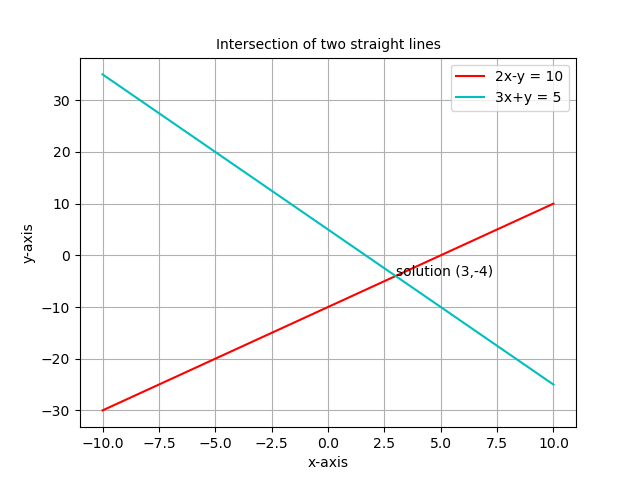
\includegraphics[width=\columnwidth]{solutions/aug/2/14/Figures/plot.png}
%          \caption{Plot of the line}
% \end{figure}

\item Given 3\myvec{x &y\\z &w}=\myvec{x &6\\-1 &2w}+\myvec{4 &x+y\\z+w &3},find the values of x,y,z and w.\\


Assume X,Y,Z,W and P are matrices of orders $2\times n$,$3 \times k$,$2\times p$,$n\times 3$ and $p\times k$,respectively.\\
Choose the correct answer in Exercise 31 and 32.\\
\item The restriction on n,k and p so that PY+WY will be defined are:\\
(A)k=3,p=n\\
 (B)k is arbitrary,p=2 \\
 (C)p is arbitrary,k=3 \\
 (D)k=2,p=3\\
\item If n=p,then the order of the matrix 7X-5Z is:\\
(A)$p \times 2$ (B)$2 \times n$ (C)$n \times 3$ (D)$p \times n$\\
\item Find the transpose of each of the following matrices:\\
(i)\myvec{5\\ \frac{1}{2} \\-1}\\ (ii)\myvec{1 &-1\\2 &3}\\ (iii)\myvec{-1 &5 &6\\\sqrt{3} &5 &6\\2 &3 &-1}\\
\item If A=\myvec{-1 &2 &3\\5 &7 &9\\-1 &1 &1} and B=\myvec{-4 &1 &-5\\1 &2 &0\\1 &3 &1},then verify that\\
(i)$(A+B)^{'}=A^{'}+B^{'}$ \\(ii) $(A-B)^{'}=A^{'}-B^{'}$\\
\solution
\begin{enumerate}
  \item 
  \item 


We clearly have,
\begin{align}
\vec{A}-\vec{B} =
\myvec{
3 & 1 & 8\\
4 & 5 & 9\\
-2 & -2 & 0}
\end{align}
Therefore 
\begin{align}
(\vec{A}-\vec{B})^\top =
\myvec{
3 & 4 & -2\\
1 & 5 & -2\\
8 & 9 & 0}\label{aug/2/16/2eq:1}
\end{align}
Now,
\begin{align}
\vec{A}^\top-\vec{B}^\top &=
\myvec{
-1 & 5 & -1\\
2 & 7 & 1\\
3 & 9 & 1}-
\myvec{
-4 & 1 & 1\\
1 & 2 & 3\\
-5 & 0 & 1}\\
\vec{A}^\top-\vec{B}^\top &=
\myvec{
3 & 4 & -2\\
1 & 5 & -2\\
8 & 9 & 0}\label{aug/2/16/2eq:2}
\end{align}
Therefore from \eqref{aug/2/16/2eq:1} and \eqref{aug/2/16/2eq:2} we can conclude that $(\vec{A}-\vec{B})^\top = \vec{A}^\top-\vec{B}^\top$.





\end{enumerate}
\item If $A^{'}$=\myvec{3 &4\\-1 &2\\0 &1} and B=\myvec{-1 &2 &1\\1 &2 &3},then verify that\\
(i) $(A+B)^{'}=A^{'}+B^{'}$ (ii)$(A-B)^{'}=A^{'}-B^{'}$
\\
\solution
\begin{enumerate}
  \item 
\begin{equation}
    \vec{B} - \vec{A} = \myvec{-3\\-5\\-3}, \vec{C} - \vec{A} = \myvec{3\\5\\13}
\end{equation}
Forming the matrix 
\begin{align}
    \vec{M} &= \myvec{
    \vec{B} -  \vec{A} & \vec{C} - \vec{A}\\
    }^\top\\
    &= \myvec{
    -3 & -5 & -3\\
    3 & 5 & 3}
\end{align}
Using matrix transformation,
\begin{align}
 \vec{M} = \myvec{
    -3 & -5 & -3\\
    3 & 5 & 3}
    \xleftrightarrow{\text{$R_2$}\rightarrow{\text{$R_2 + R_1$ }}}
 \myvec{
 -3 & -5 & -3\\
 0 & 0 & 0}\
\end{align}
\begin{equation}
   \implies rank(\vec{M}) = 1 
\end{equation}
Thus $\vec{A}$, $\vec{B}$ and $\vec{C}$ are collinear.
% \begin{figure}[!h]
%          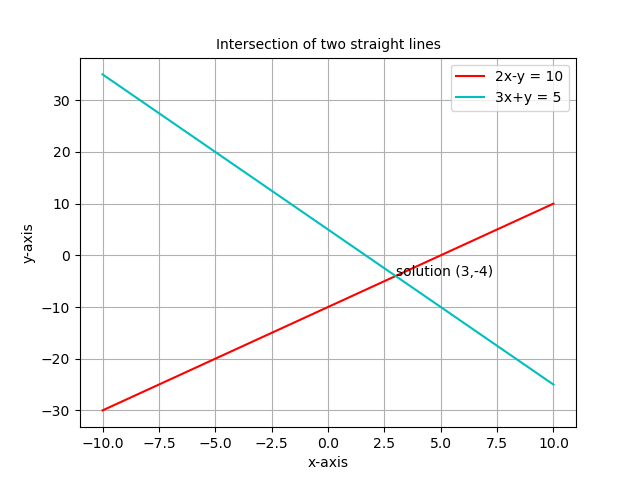
\includegraphics[width=\columnwidth]{solutions/aug/2/14/Figures/plot.png}
%          \caption{Plot of the line}
% \end{figure}

  \item 
\end{enumerate}

\item If$ A^{'}$=\myvec{-2 &3\\1 &2} and B=\myvec{-1 &0\\1 &2},then find that $(A+2B)^{'}$\\

  \item (i) Show that the matrix A=\myvec{1 &-1&5\\-1 &2 &1\\5 &1 &3} is a symmetric matrix.\\
  (ii) Show that the matrix A=\myvec{0 & 1 &-1\\-1 &0 &1\\1&-1 &0} is a skew symmetric matrix.\\
  \solution
  \begin{enumerate}
    \item Given,
    \begin{align}
    \label{aug/2/19/eq:1}
        \vec{A}=\myvec{1 & -1 & 5\\ -1 & 2 & 1\\5 & 1 & 3}
    \end{align}
    Transposing the matrix,
    \begin{align}
        \label{aug/2/19/eq:2}
        \vec{A}^\top=\myvec{1 & -1 & 5 \\-1 & 2 & 1\\5 & 1 &3}
    \end{align}
    Using \eqref{aug/2/19/eq:1} and \eqref{aug/2/19/eq:2} we get,
    \begin{align}
        \vec{A}=\vec{A}^\top
    \end{align}
    %\begin{center}
        $\therefore \vec{A}$ is symmetric matrix. 
    %\end{center}
        
    \item Given,
    \begin{align}
    \label{aug/2/19/eq:4}
        \vec{A}=\myvec{0 & 1 & -1\\ -1 & 0 & 1\\1 & -1 & 0}
    \end{align}
    Transposing the matrix,
    \begin{align}
        \label{aug/2/19/eq:5}
        \vec{A}^\top=\myvec{0 & -1 & 1 \\1 & 0 & -1\\-1 & 1 & 0}
    \end{align}
    Using \eqref{aug/2/19/eq:4} and \eqref{aug/2/19/eq:5} we get,
    \begin{align}
        \vec{A}=-\vec{A}^\top
    \end{align}
    %\begin{center}
        $\therefore \vec{A}$ is skew symmetric matrix. 
    %\end{center}
    \end{enumerate}
  \item For the matrix A=\myvec{1 &5\\6 &7},verify that\\
  (i)$(A+A^{'})$ is a symmetric matrix\\
  (ii)$(A-A^{'})$ is a skew symmetric matrix\\
  
  \item Find $\frac{1}{2}(A+A^{'}) $and $\frac{1}{2}(A-A^{'})$,when A=\myvec{0 &a &b\\-a &0 &c\\-b &-c &0}\\
  \item Express the following matrices as the sum of a symmetric and a skew symmetric matrix:\\
  (i) \myvec{3 &5\\1 &1} \\(ii) \myvec{6 &-2 &2\\-2 &3 &-1\\2 &-1 &3} \\
  (iii) \myvec{3 &3 &-1\\-2 &-2 &1\\-4 &-5 &2}\\ (iv) \myvec{1 &5\\-1 &2}\\
  \begin{enumerate}
    \item 
Let the given Matrix be
\begin{equation}
\vec{A} = \myvec{3&5\\1&1}
\end{equation}
Transposing the above matrix gives,
\begin{equation}
\vec{A}^{\top} = \myvec{3&1\\5&1}
\end{equation}
Now, for Symmetric and Skew Symmetric Matrix,
\begin{align}
    \vec{B} &= \frac{\vec{A} + \vec{A}^{\top}}{2} = \myvec{3&3\\3&1} \\
    &= \vec{B}^{\top}
\end{align}
Also,
\begin{align}
    \vec{C} &= \frac{\vec{A} - \vec{A}^{\top}}{2} = \myvec{0&2\\-2&0} \\
    &= -\vec{C}^{\top}
\end{align}

Hence, $\vec{B}$ is a Symmetric Matrix and $\vec{C}$ is a Skew Symmetric Matrix and $\vec{B} + \vec{C} = \vec{A}$.
\begin{align}
    \therefore \myvec{3&5\\1&1} = \myvec{3&3\\3&1} + \myvec{0&2\\-2&0}  
\end{align}




  \end{enumerate}
  Choose the correct answer in question number 43 and 44\\
  \item If A,B are symmetric matrices of same order,then AB-BA is a\\
  (A)Skew symmetric matrix \\(B)Symmetric matrix\\
  (C)Zero matrix \\ (D)Identity matrix\\
  
  
  \item\myvec{1 &3\\2 &7}\\
  \item\myvec{2 &3\\5 &7}\\
  \item\myvec{2 &1\\7 &4}\\
  \item \myvec{2 &5\\1 &3}\\
  \item \myvec{3 &1\\5 &2}\\
  \item \myvec{4 &5\\3 &4}\\
  \item \myvec{3 &10\\2 &7}\\
  \item \myvec{3 &-1\\-4 &2}\\
  \item \myvec{2 &-6\\1 &-2}\\
  \item \myvec{6 &-3\\-2 &1}\\
  \item \myvec{2 &-3\\-1 &2}\\
  \item \myvec{2 &1\\4 &2}\\
  
  \item Matrices Aand B will be inverse of each other only if\\
  (A)AB=BA (B)AB=BA=0\\
  (C)AB=0,BA=I (D)AB=BA=I\\
  
  \item Let A=\myvec{0 &1\\0 &0},show that \\$(aI+bA)^{n}=a^{n}I+na^{n-1}bA$,where I is the identity matrix of order 2 and $n \epsilon N$\\

  \item If A and B are symmetric matrices,prove that AB-BA is a skew symmetric matrix.\\
  
  \item If A and B are square matrices of the same order such that AB=BA,then prove by indication that $AB^{n}=B^{n}A$.Further prove that $(AB)^{n}=A^{n}B^{n}$ for all $n \epsilon N$.\\
  Choose the correct answer in the following questions:\\

\item Balance the following chemical equation
\begin{align}\label{1}
    BaCl_2 + H_2SO_4 \xrightarrow{} BaSO_4 + HCl
\end{align}
    \item If A=\myvec{1 &2 &3\\2 &3 &1} and B=\myvec{3 &-1 &3\\-1 &0 &2}, then find 2A-B.\\
    \item If A=\myvec{8 &0\\4 &-2\\3 &6} and B=\myvec{2 &-2\\4 &2\\-5 &1}, then find the matrix X, such that 2A+3X=5B.\\
    \item Find X and Y, if X+Y=\myvec{5 &2\\0 &9} and \\X-Y=\myvec{3 &6\\0 &-1}.\\
    \item Find the values of x and y from the following equation:\\
    2\myvec{x &5\\7 &y-3} + \myvec{3 &-4\\1 &2} = \myvec{7 &6\\15 &14}\\
     
    

   
    \item  Find AB, if A=\myvec{6 &9\\2 &3} and B=\myvec{2 &6 &0\\7 &9 &8}.\\
    \item  If A=\myvec{1 &-2 &3\\-4 &2 &5\\} and B=\myvec{2 &3\\4 &5\\2 &1}, then find AB,BA.Show that AB$\neq$BA

   
     \item If A=\myvec{1 &0 \\0 &-1} and  B=\myvec{0 &1\\1 &0}, then find AB,BA. Show that AB$\neq$BA\\
     
   
    \item Find AB, if A=\myvec{0 &-1\\0 &2} and B=\myvec{3 &5\\0 &0}\\
    \solution $AB = 0$.

     
   
    \item If A=\myvec{1 &1 &-1\\2 &0 &3\\3 &-1 &2}, B=\myvec{1 &3\\0 &2\\-1 &4} and C=\myvec{1 &2 &3 &-4\\2 &0 &-2 &1}, find\\A(BC),(AB)C and show that (AB)C=A(BC) \\   
    
     \item If A=\myvec{0 &6 &7\\-6 &0 &8\\7 &-8 &0}, B=\myvec{0 &1 &1\\1 &0 &2\\1 &2 &0},C=\myvec{2\\-2\\3}\\Calculate AC,BC and (A+B)C=AC+BC\\
     \solution
     \begin{align}
    \vec{AC}&=\myvec{0&6&7\\-6&0&8\\7&-8&0}\myvec{2\\-2\\3}\\
  &=\myvec{9\\12\\30}
\end{align}
\begin{align}
    \vec{BC}&=\myvec{0&1&1\\1&0&2\\1&2&0}\myvec{2\\-2\\3}\\
  &=\myvec{1\\8\\-2}
\end{align}
Now,
\begin{align}
    \vec{AC}+\vec{BC}&=\myvec{9\\12\\30}+\myvec{1\\8\\-2}\\
    &=\myvec{10\\20\\28} \label{aug/50/eq-2}
\end{align}
and,
\begin{align}
    (\vec{A}+\vec{B})\vec{C}&=\myvec{0&7&8\\-5&0&10\\8&-6&0}\myvec{2\\-2\\3}\\
&=\myvec{10\\20\\28} \label{aug/50/eq-1}
\end{align}
From \eqref{aug/50/eq-1} and \eqref{aug/50/eq-2},
\begin{align}
    (\vec{A}+\vec{B})\vec{C}=\vec{AC}+\vec{BC}
\end{align}

    
    

\item If A=$\myvec{3 &\sqrt{3} &2\\4 &2 &0}$ and B=$\myvec{2 &-1 &2\\1 &2 &4}$, verify that\\
(i) $(A^{'})^{'}=A$\\ (ii)$(A+B)^{'}=A^{'}+B^{'}$,\\ (iii) $(kB)^{'}=kB^{'}$,where k is any constant.\\
\item If A=$\myvec{-2\\4 \\5}$,B=$\myvec{1 &3 &-6}$, verify that $(AB)^{'}=B^{'}A^{'}$\\
  
\item By using elementary operations,find the inverse of the matrix\\
A=$\myvec{1 &2\\2 &-1}$.\\

\item If A=$\myvec{\cos\theta &\sin\theta\\ \-sin\theta &\cos\theta}$,\\then prove that $A^{n}=\myvec{\cos\theta &\sin n\theta\\\-sin n\theta &\cos n\theta}$, n $\in$ N.\\
\item If A and B are symmetric matrices of the same order, then show that AB is symmetric if and only if A and B commute,that AB = BA.\\
\item Let A=$\myvec{2 &-1\\3 &4}$, B=$\myvec{5 &2\\7 &4}$, C=$\myvec{2 &5\\3 &8}$. Find a matrix D such that CD-AB=0. 
\item Find the values of a,b,c and d from the equations: \myvec{a-b &2a+c\\2a-b &3c+d} = \myvec{-1 &5\\0 &13}
\item Show that\\
(i)$\myvec{5 &-1\\6 &7}\myvec{2 &1\\3 &4}\neq\myvec{2 &1\\3 &4}\myvec{5 &-1\\6 &7}$
\\
(ii)$\myvec{1 &2 &3\\0 &1 &0\\1 &1 &0}\myvec{-1 &1 &0\\0 &-1 &1\\2 &3 &4}\neq \myvec{-1 &1 &0\\0 &-1 &1\\2 &3 &4}\myvec{1 &2 &3\\0 &1 &0\\1 &1 &0}$\\
\item If A=\myvec{3 &-2\\4 &-2} and I=\myvec{1 &0\\0 &1},find k\\
 so that $A^2=kA-2I$\\
  \item Find the matrix X so that\\ X\myvec{1 &2 &3\\4 &5 &6}=\myvec{-7 &-8 &-9\\2 &4 &6}\\
\item (i) $\begin{vmatrix}a-b-c& 2a& 2a \\ 2b& b-c-a& 2b \\ 2c& 2c& c-a-b\end{vmatrix}$= $(a+b+c)^3$\\
(ii) $\begin{vmatrix}x+y+2z&x&y \\ z&y+z+2x&y \\ z&x&z+x+2y\end{vmatrix}$=$2(x+y+z)^3$
\item $\begin{vmatrix}1&x&x^2 \\ x^2&1&x \\ x&x^2&1\end{vmatrix}$=$(1-x^3)^2$ 
\item $\begin{vmatrix}1+a^2-b^2&2ab&-2b \\ 2ab&1-a^2+b^2&2a \\ 2b&-2a&1-a^2-b^2\end{vmatrix}$=$(1+a^2+b^2)^3$
\item Let 
A=$\begin{bmatrix}
1&\sin\theta&1 \\ -\sin\theta&1&\sin\theta \\ -1&-\sin\theta&1
\end{bmatrix},$ 
where $0\leq \theta \leq 2\Pi.$ Then
\begin{enumerate}
\item Det(A)=0
\item Det(A)$\in(2,\infty)$
\item Det(A)$\in (2,4)$
\item Det(A)$\in [2,4]$
\end{enumerate}
\item $\begin{vmatrix}
1&1+p&1+p+q \\ 2&3+2p&4+3p+2q \\ 3&6+3p&10+6p+3q
\end{vmatrix}$=1\\
\item $\begin{vmatrix}\sin\alpha&\cos\alpha&\cos(\alpha+\delta) \\ \sin\beta&\cos\beta&\cos(\beta+\delta) \\ \sin\gamma&\cos\gamma&\cos(\gamma+\delta)\end{vmatrix}$=0\\
\item Solve the system of equations \\$\frac{2}{x}+\frac{3}{y}+\frac{10}{z}=4$\\$\frac{4}{x}-\frac{6}{y}+\frac{5}{z}=1$\\$\frac{6}{x}+\frac{9}{y}-\frac{20}{z}=2$\\
\item If a,b,c are in A.P, then the determinant\\
 $\begin{vmatrix}
x+2&x+3&x+2a \\ x+3&x+4&x+2b \\x+4&x+5&x+2c
\end{vmatrix}$ is 
\begin{enumerate}
\item 0
\item 1
\item x
\item 2x
\end{enumerate}
\item If x,y,z are nonzero real numbers, then the inverse of matrix 
A=$\begin{bmatrix}
x&0&0 \\ 0&y&0 \\ 0&0&z
\end{bmatrix}$ is 
\begin{enumerate}
\item $\begin{bmatrix} x^{-1}&0&0 \\ 0&y^{-1}&0 \\ 0&0&z^{-1} \end{bmatrix}$ 
\item $xyz\begin{bmatrix} x^{-1}&0&0 \\ 0&y^{-1}&0 \\ 0&0&z^{-1} \end{bmatrix}$ 
\item $\frac{1}{xyz}\begin{bmatrix} x&0&0 \\ 0&y&0 \\ 0&0&z \end{bmatrix}$ 
\item $\frac{1}{xyz}\begin{bmatrix} 1&0&0 \\ 0&1&0 \\ 0&0&1 \end{bmatrix}$ 
\end{enumerate}
\textbf{Examine the consistency of the system of given Equations.}
\item 
$\begin{alignedat}[t]{2}
x+2y&=2 
\\
2x+3y&=3 
\end{alignedat}$
\item $\begin{alignedat}[t]{2}
2x-y&=5 
\\
x+y&=4 
\end{alignedat}$
\item Evaluate the determinant
$\begin{vmatrix}0&a&-b\\-a&0&-c\\b&c&0\end{vmatrix}=0$
\\
Find the inverse and QR decomposition of the following.
  \item \myvec{2 &1\\1 &1}\\
  \item\myvec{1 &3\\2 &7}\\
  \item\myvec{2 &3\\5 &7}\\
  \item\myvec{2 &1\\7 &4}\\
  \item \myvec{2 &5\\1 &3}\\
  \item \myvec{3 &1\\5 &2}\\
  \item \myvec{4 &5\\3 &4}\\
  \item \myvec{3 &10\\2 &7}\\
  \item \myvec{3 &-1\\-4 &2}\\
  \item \myvec{2 &-6\\1 &-2}\\
  \item \myvec{6 &-3\\-2 &1}\\
  \item \myvec{2 &-3\\-1 &2}\\
  \item \myvec{2 &1\\4 &2}\\
\item Find the QR decomposition of 
\begin{align}
\vec{A}=\myvec{8&5\\3&2} \label{eq:solutions/decomp/2/29/eq:1}
\end{align}
%%
%
\item Find the QR decomposition of 
\begin{align}
\vec{A}=\myvec{2&5\\1&4} \label{eq:solutions/decomp/2/30/1}
\end{align}

%    \end{document}    



\end{enumerate}

%
%
\end{document}


